\documentclass[tikz,border=4pt]{standalone}
\usepackage[T1]{fontenc}
\usepackage{lmodern}
\usepackage{amsmath}
% Shared TikZ style for the report figures.
% Colours follow the Okabe-Ito palette, which stays distinguishable under the
% common forms of colour-vision deficiency. Every colour-coded element also
% carries a text label, so no figure depends on colour alone.
\usetikzlibrary{arrows.meta,positioning,fit,calc,backgrounds,decorations.pathreplacing,shapes.geometric}

\definecolor{oiOrange}{HTML}{E69F00}
\definecolor{oiSky}{HTML}{56B4E9}
\definecolor{oiGreen}{HTML}{009E73}
\definecolor{oiYellow}{HTML}{F0E442}
\definecolor{oiBlue}{HTML}{0072B2}
\definecolor{oiVerm}{HTML}{D55E00}
\definecolor{oiPurple}{HTML}{CC79A7}
\definecolor{oiGray}{HTML}{6E6E6E}

\colorlet{corTreino}{oiBlue!22}
\colorlet{corValid}{oiGreen!30}
\colorlet{corTeste}{oiOrange!45}
\colorlet{corControle}{oiPurple!35}

\tikzset{
  >=Stealth,
  bloco/.style={draw=black!70, rounded corners=1.5pt, minimum height=0.62cm,
    inner sep=2pt, font=\sffamily\fsz, align=center},
  treino/.style={bloco, fill=corTreino},
  valid/.style={bloco, fill=corValid},
  teste/.style={bloco, fill=corTeste, thick},
  etapa/.style={draw=black!70, rounded corners=3pt, fill=black!4,
    text width=4.3cm, align=center, inner sep=4pt, font=\sffamily\fsz},
  nota/.style={font=\sffamily\fsz, align=left, text=black!80},
  titulo/.style={font=\sffamily\fst\bfseries, anchor=west},
  seta/.style={->, thick, black!70},
  regiao/.style={draw=black!50, dashed, rounded corners=4pt},
}

% Absolute font sizes, so a figure looks the same standalone (10 pt class) and
% inside the 11 pt report.
\providecommand{\fsx}{\fontsize{5.5}{6.5}\selectfont}
\providecommand{\fsz}{\fontsize{7}{8.5}\selectfont}
\providecommand{\fst}{\fontsize{9}{11}\selectfont}

\begin{document}
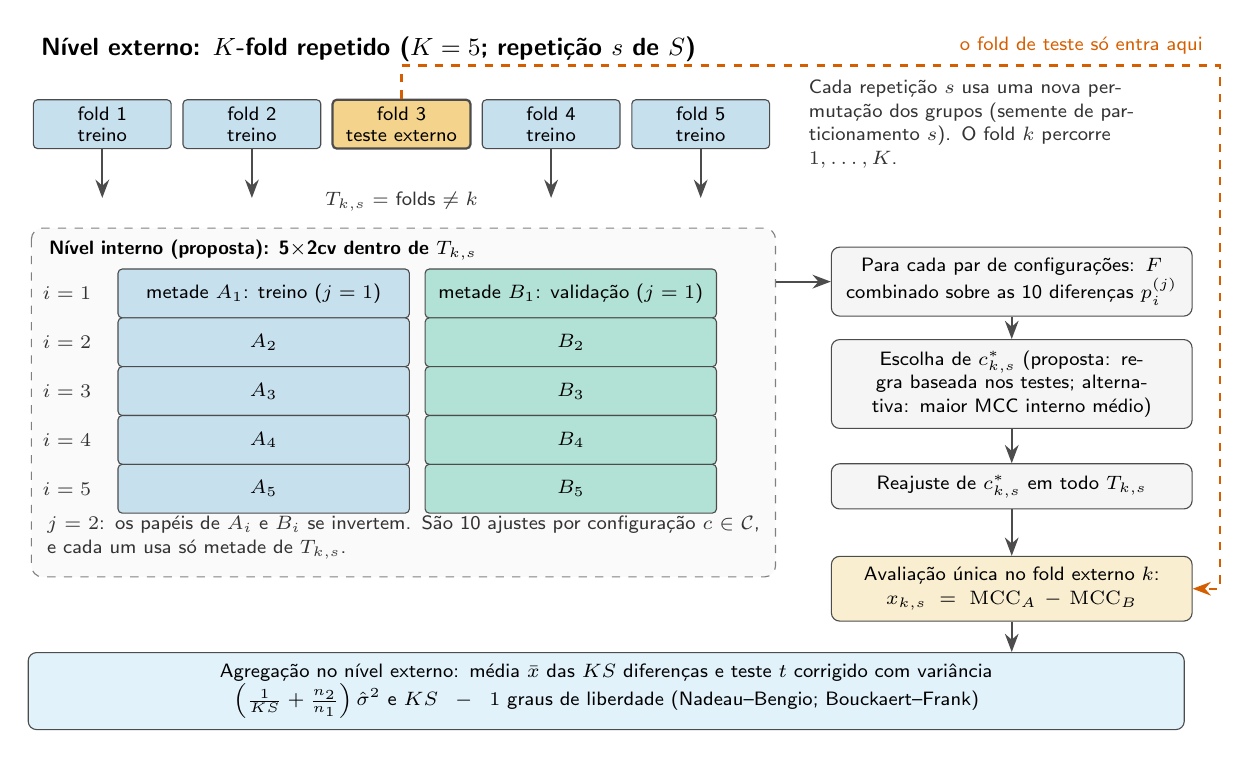
\begin{tikzpicture}
  % ---- Outer level: one repetition s of K-fold ----
  \node[titulo] at (0,0.95) {Nível externo: $K$-fold repetido ($K=5$; repetição $s$ de $S$)};
  \foreach \k/\x in {1/0.9,2/2.8,3/4.7,4/6.6,5/8.5} {
    \ifnum\k=3
      \node[teste, minimum width=1.75cm] (f\k) at (\x,0) {fold \k\\[-1pt]teste externo};
    \else
      \node[treino, minimum width=1.75cm] (f\k) at (\x,0) {fold \k\\[-1pt]treino};
    \fi
  }
  \node[nota, anchor=west, text width=4.6cm] at (9.75,0)
    {Cada repetição $s$ usa uma nova permutação dos grupos (semente de particionamento $s$). O fold $k$ percorre $1,\dots,K$.};
  \foreach \k in {1,2,4,5} { \draw[seta] (f\k.south) -- ++(0,-0.62); }
  \node[nota, fill=white, inner sep=1pt] at (4.7,-0.98) {$T_{k,s}$ = folds $\neq k$};

  % ---- Inner level: 5x2cv inside T_{k,s} ----
  \draw[regiao, fill=black!2] (0,-1.32) rectangle (9.45,-5.75);
  \node[titulo, font=\sffamily\fsz\bfseries] at (0.1,-1.6)
    {Nível interno (proposta): 5$\times$2cv dentro de $T_{k,s}$};
  \foreach \i in {1,...,5} {
    \pgfmathsetmacro\y{-2.15-0.62*(\i-1)}
    \node[nota] at (0.45,\y) {$i=\i$};
    \ifnum\i=1
      \node[treino, minimum width=3.7cm] at (2.95,\y) {metade $A_1$: treino ($j=1$)};
      \node[valid,  minimum width=3.7cm] at (6.85,\y) {metade $B_1$: validação ($j=1$)};
    \else
      \node[treino, minimum width=3.7cm] at (2.95,\y) {$A_\i$};
      \node[valid,  minimum width=3.7cm] at (6.85,\y) {$B_\i$};
    \fi
  }
  \node[nota, text width=9.1cm] at (4.75,-5.25)
    {$j=2$: os papéis de $A_i$ e $B_i$ se invertem. São 10 ajustes por configuração $c\in\mathcal{C}$, e cada um usa só metade de $T_{k,s}$.};

  % ---- Selection and evaluation flow ----
  \node[etapa] (e1) at (12.45,-2.0) {Para cada par de configurações: $F$ combinado sobre as 10 diferenças $p_i^{(j)}$};
  \node[etapa] (e2) at (12.45,-3.3) {Escolha de $c^\ast_{k,s}$ (proposta: regra baseada nos testes; alternativa: maior MCC interno médio)};
  \node[etapa] (e3) at (12.45,-4.6) {Reajuste de $c^\ast_{k,s}$ em todo $T_{k,s}$};
  \node[etapa, fill=corTeste!40] (e4) at (12.45,-5.9) {Avaliação única no fold externo $k$:\\ $x_{k,s}=\mathrm{MCC}_A-\mathrm{MCC}_B$};
  \draw[seta] (9.45,-2.0) -- (e1.west);
  \draw[seta] (e1) -- (e2);
  \draw[seta] (e2) -- (e3);
  \draw[seta] (e3) -- (e4);
  \draw[seta, dashed, oiVerm] (f3.north) -- ++(0,0.42) -| ($(e4.east)+(0.35,0)$) -- (e4.east);
  \node[nota, text=oiVerm, anchor=south east] at (15.0,0.76) {o fold de teste só entra aqui};

  % ---- Aggregation ----
  \node[etapa, text width=14.4cm, fill=oiSky!18] (ag) at (7.3,-7.2)
    {Agregação no nível externo: média $\bar{x}$ das $KS$ diferenças e teste $t$ corrigido com variância $\left(\frac{1}{KS}+\frac{n_2}{n_1}\right)\hat{\sigma}^2$ e $KS-1$ graus de liberdade (Nadeau--Bengio; Bouckaert--Frank)};
  \draw[seta] (e4.south) -- (e4.south |- ag.north);
\end{tikzpicture}
\end{document}
